% Model 1 daily water bucket (one daily step). Same colours as m1_two_clocks.
% Build: cd Paper/Figure && pdflatex m1_bucket.tex
\documentclass[tikz,border=4pt]{standalone}
\usepackage{newtxtext,newtxmath}
\usepackage{amsmath}
\usetikzlibrary{arrows.meta,decorations.pathreplacing,calc}
\definecolor{dy}{HTML}{2B6CB0}   % water
\definecolor{yr}{HTML}{18473C}   % plants / cover
\definecolor{leaf}{HTML}{3EBA91}
\definecolor{lim}{HTML}{D64545}  % limits: red dashed
\definecolor{ink}{HTML}{333333}
\begin{document}
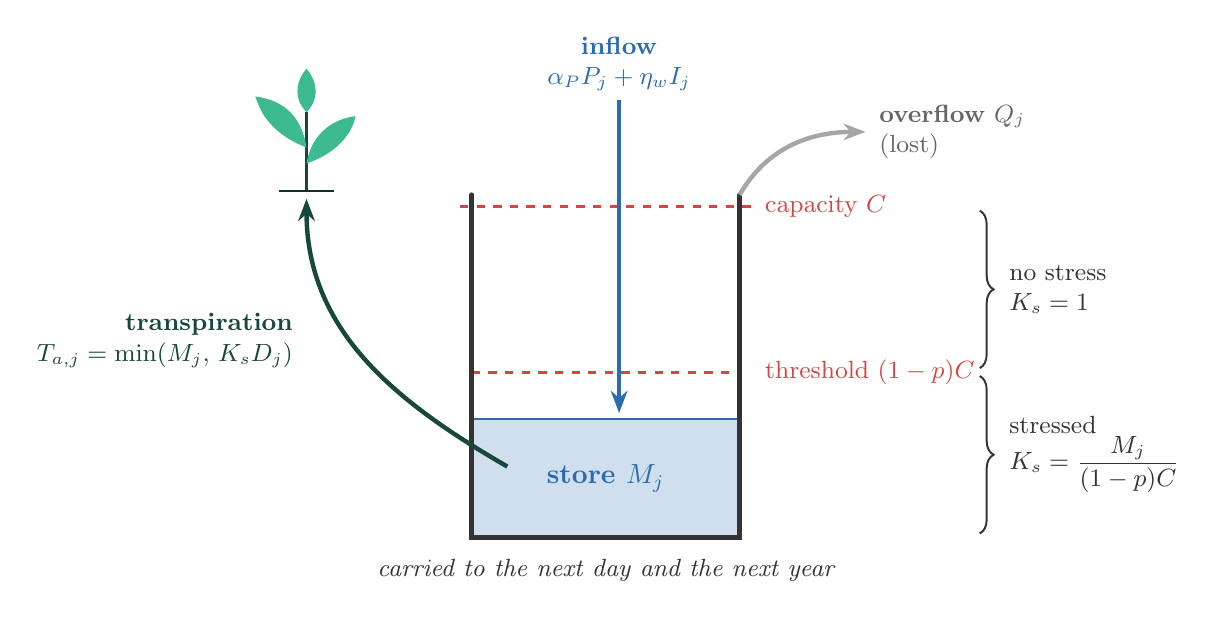
\begin{tikzpicture}[font=\normalsize,
  flow/.style={-{Stealth[length=8pt,width=6pt]}, line width=1.6pt},
  limit/.style={lim, dashed, line width=1.1pt}]
\def\W{3.4}\def\H{4.2}\def\Thr{2.1}\def\Lvl{1.5}
% ---- water and bucket ----
\fill[dy!22] (0,0) rectangle (\W,\Lvl);
\draw[dy, line width=0.8pt] (0,\Lvl) -- (\W,\Lvl);
\node[dy, font=\normalsize\bfseries] at (\W/2,\Lvl/2) {store $M_j$};
\draw[limit] (-0.15,\H) -- (\W+0.15,\H);
\draw[limit] (0,\Thr) -- (\W,\Thr);
\draw[ink, line width=1.8pt, line cap=round] (0,\H+0.15) -- (0,0) -- (\W,0) -- (\W,\H+0.15);
% ---- line labels (right) and stress zones (brace) ----
\node[lim, anchor=west, font=\small] at (\W+0.2,\H) {capacity $C$};
\node[lim, anchor=west, font=\small] at (\W+0.2,\Thr) {threshold $(1-p)C$};
\draw[decorate, decoration={brace, amplitude=5pt}, ink, line width=0.7pt] (\W+3.05,\H-0.05) -- (\W+3.05,\Thr+0.05)
  node[midway, right=7pt, align=left, font=\small, text=ink] {no stress\\$K_s=1$};
\draw[decorate, decoration={brace, amplitude=5pt}, ink, line width=0.7pt] (\W+3.05,\Thr-0.05) -- (\W+3.05,0.05)
  node[midway, right=7pt, align=left, font=\small, text=ink] {stressed\\$K_s=\dfrac{M_j}{(1-p)C}$};
% ---- inflow (top) ----
\draw[flow, dy] (\W*0.55,\H+1.35) -- (\W*0.55,\Lvl+0.08);
\node[dy, anchor=south, font=\small, align=center] at (\W*0.55,\H+1.35) {\textbf{inflow}\\$\alpha_P P_j+\eta_w I_j$};
% ---- overflow (top right) ----
\draw[flow, gray!70] (\W,\H+0.15) to[out=60, in=180] (\W+1.6,\H+0.95);
\node[gray!80!black, anchor=west, font=\small, align=left] at (\W+1.65,\H+0.95) {\textbf{overflow} $Q_j$\\(lost)};
% ---- plant and transpiration (left) ----
\begin{scope}[shift={(-2.1,\H+0.2)}]
  \draw[yr, line width=1.4pt] (0,0) -- (0,1.0);
  \fill[leaf] (0,0.55) .. controls (-0.5,0.75) and (-0.6,1.05) .. (-0.65,1.2) .. controls (-0.25,1.15) and (-0.05,0.9) .. (0,0.55);
  \fill[leaf] (0,0.35) .. controls (0.45,0.5) and (0.6,0.8) .. (0.62,0.95) .. controls (0.25,0.9) and (0.05,0.65) .. (0,0.35);
  \fill[leaf] (0,1.0) .. controls (-0.2,1.2) and (-0.1,1.45) .. (0,1.55) .. controls (0.1,1.45) and (0.2,1.2) .. (0,1.0);
  \draw[yr!70!black, line width=0.6pt] (-0.35,0) -- (0.35,0);
\end{scope}
\draw[flow, yr] (0.45,\Lvl*0.6) to[out=150, in=-90] (-2.1,\H+0.1);
\node[yr, anchor=east, font=\small, align=right] at (-2.15,\H-1.7) {\textbf{transpiration}\\$T_{a,j}=\min(M_j,\,K_sD_j)$};
% ---- carry-over note ----
\node[ink, font=\small\itshape, anchor=north] at (\W/2,-0.15) {carried to the next day and the next year};
\end{tikzpicture}
\end{document}
